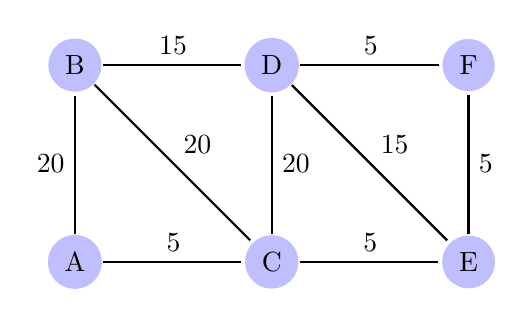
\begin{tikzpicture}[shorten >=1pt,auto,node distance=2.5cm,thick,main node/.style={circle,fill=blue!25}]                      
  \node[main node] (F) {F};                
  \node[main node] (D) [left of=F] {D};    
  \node[main node] (E) [below of=F] {E};   
  \node[main node] (B) [left of=D] {B};    
  \node[main node] (C) [below of=D] {C};   
  \node[main node] (A) [below of=B] {A};   
              
	\path[-, draw, thick]
  (A) edge node {$20$} (B)
	(B) edge node {$20$} (C)
	(B) edge node {$15$} (D)
	(C) edge node[right] {$20$} (D)
	(C) edge node {$5$} (E)
	(D) edge node {$15$} (E)
	(D) edge node {$5$} (F)
	(E) edge node[right] {$5$} (F)
	(A) edge node {$5$} (C)
	;
\end{tikzpicture}
